\documentclass[12pt,letterpaper]{article}
\usepackage[utf8]{inputenx} %Codificacion del texto (ISO Latin1 encoding)

\usepackage{fancyhdr} %Permite acomodar a tu gusto la parte de arriba y
% abajo del documento
\usepackage[spanish]{babel} %Permite definir el idioma del dcumento
\usepackage{graphicx} %Permite exportar imagenes en formato eps
\usepackage{hyperref}
\usepackage{url} %Tipo de fuente para correos y paginas
\usepackage{pgf}
\usepackage{fleqn}
\usepackage{amssymb}
\usepackage{amsmath}
\usepackage{fancyvrb}
\usepackage{makeidx}
\usepackage{multirow}
\usepackage{colortbl} %Permite colocar colores a las tablas
\usepackage{booktabs}
\usepackage[final]{pdfpages}
%%%%%%%%%%
%Margenes%
%%%%%%%%%%
\parskip 1mm %Espacio entre parrafos

\setlength{\topmargin}{0pt}
\topmargin      0.5cm
\oddsidemargin	0.1cm  % Ancho Letter 21,59cm
\evensidemargin 0.5cm  % Alto  Letter 27,81cm
\textwidth	17cm%15.5cm
\textheight	21.0cm
\headsep	4 mm
\parindent	1.2cm
%%%%%%%%%%%%%%%%%%%%%%
%Estilo del documento%
%%%%%%%%%%%%%%%%%%%%%%
\pagestyle{fancyplain}

%%%%%%%%%%%%%%%%%%%%%%%%%%%%%%%%%%%%%%%%%%%
%Fancyheadings. Top y Bottom del documento%
%%%%%%%%%%%%%%%%%%%%%%%%%%%%%%%%%%%%%%%%%%%
% Recuerde que en este documento la portada del documento no posee
% numeracion, pero de igual manera llamaremos a esa primera pagina la numero
% 1, y la que viene la dos. Esto es para tener una idea de las que
% llamaremos pares e impares
\lhead{Innovación Tecnológica} %Parte superior izquierda
\rhead{\bf \it Departamento de Informática - UTFSM} %Parte superior derecha
\lfoot{\it Analytic Network Process} %Parte inferior izquierda. \thepage indica
% el numero de pagina
\cfoot{} %Parte inferior central
\rfoot{\bf \thepage} %Parte inferior derecha
\renewcommand{\footrulewidth}{0.4pt} %Linea de separacion inferior

\newcommand{\primaria}[1]{
	\textbf{\underline{#1}}
}

\newcommand{\foranea}[1]{
	\textbf{\textsl{#1}}
}

\newcommand{\primyfor}[1]{
	\underline{\foranea{#1}}
}

\makeatletter
\newcommand\subsubsubsection{\@startsection {paragraph}{1}{\z@}%
                                   {-3.5ex \@plus -1ex \@minus -.2ex}%
                                   {1.5ex \@plus.2ex}%
                                   {\normalfont\bfseries}}
\newcommand\subsubsubsubsection{\@startsection {subparagraph}{1}{\z@}%
                                   {-3.5ex \@plus -1ex \@minus -.2ex}%
                                   {1.5ex \@plus.2ex}%
                                   {\normalfont\bfseries}}


\makeatother
\makeindex

\begin{document}
\begin{titlepage}
\title{Analytic Network Process \\ \begin{Large}\it Una Estimación del Mejor Proveedor para Natural Response\end{Large}} 
\author{\emph{Autor:}\\Victor Gonzalez Rodriguez\\\url{victor.gonzalezr@usm.cl} \\
\and \emph{Profesor:}\\Lautaro Guerra\\\url{lautaro.guerra@usm.cl}}
\date{\today}
\maketitle

\begin{abstract}
El mercado de los proveedores de Natural Response, es un mercado altamente dinámico, donde cada proveedor disponible lucha por vender sus productos a empresas como Natural Response. Por esta razón, a Natural Response le interesa saber cuales son sus mejores opciones dentro del amplio mercado de proveedores tanto nacionales como internacionales. Si consideramos todas las condiciones que Natural Response presenta, el problema se ajusta muy bien a la estructura del Analytic Network Process, por lo que se desarrolló un modelo basado en este método para así estimar y entender mejor cuales son las mejores opciones de proveedores para Natural Response. Los criterios más relevantes para la elección de un proveedor para esta empresa son: relación comercial, calidad, costos, sensibilidad/comprensión y despacho. Los resultados fueron validados al comparar las estimaciones del modelo ANP con las estimaciones realizadas por el estudio periódico que realiza la empresa. Los resultados indican que el modelo representa de manera acertada la realidad de la empresa en cuanto se trata de evaluar proveedores, por lo que Natural Response se ha mostrado interesado en implementar este modelo en su análisis de incorporación y evaluación periódica de proveedores.
\end{abstract}
\end{titlepage}
\newpage
\tableofcontents
\newpage

\section{Introducción}
La empresa Natural es una empresa jóven, dinámica y con mucho crecimiento año a año, la cual la ha posicionado internacionalmente como una de las mejores empresas a nivel mundial en la extracción sustentable de productos naturales obtenidos de la flora chilena, tales como el quillay. Es por esto, que la empresa maneja cada vez más proveedores que le entreguen sus materias primas para el desarrollo de sus productos, con una base de datos de proveedores autorizados que bordea la cifra de los 60, y con una cantidad de más de 80 proveedores que está a la espera de ser autorizado para colaborar con Natural Response. Es por esto, que se ha hecho necesario establecer una métrica que le permita a la empresa saber que empresa está cumpliendo de mejor manera los criterios que Natural Response estima pertinentes, ya que la empresa espera producir con estándares de alta calidad, que le permitan posicionarse de manera estable en el mercado mundial.\\

En la actualidad, Natural Response utiliza un símil a lo que se conoce como Analytic Hierarchy Process, donde se tiene un sistema de calificación de proveedores a partir de 5 criterios, almacenados en una plantilla Excel con más de 80 libros. Si bien este modelo está funcionando de buena manera, se puede obtener un mejor modelo que permita entender de que manera la empresa necesita priorizar las características que debe tener un proveedor que quiere ser autorizado, o se quiere mantener autorizado.\\

El método que nos permite entender ``Cual es el mejor proveedor para Natural Response'', es claramente el método Analytic Network Process, basado en el análisis de \textit{Beneficios, Costos y Riesgos}, donde podemos comparar una cantidad limitada de proveedores.\\
Para esto, supondremos que 4 proveedores actualmente autorizados, son proveedores que están a la espera de ingresar a la lista de proveedores autorizados, y que veremos cual de ellos merece ingresar, y los datos se validarán comparando con la evaluación periódica de proveedores que nos ha facilitado la empresa Natural Response. Además, utilizaremos el programa \textit{Super Decisions Software\footnote{\url{http://www.superdecisions.com/}}}, desarrollado por el \textit{Creative Decisions Foundation}, basandose en la teoría creada por Thomas L. Saaty sobre el Analytic Network Process, el cual nos permitirá facilitar el trabajo y los pasos necesarios para realizar el análisis del método que estudiaremos.
\newpage

\section{El método Analytic Network Process}
\subsection{Definición}
El Analytic Network Process (ANP), es una generalización del Analytic
Hierarchy Process (AHP) utilizado en el análisis de decisiones multi-criterio. Es un método realizado por el matemático y analista Thomas L. Saaty, ha probado ser un método robusto y ampliamente usado por empresas y gobiernos\footnote{El 2005, un libro citó ejemplos de los Estados Unidos, Brasil, Chile, República Checa, Alemania, India, Indonesia, Italia, Korea, Polonia, Rusia, España, Taiwan y Turkia.} a nivel de evaluación de las tecnologías de la información (TIC).\\

Por un lado, el AHP toma la decisión de problemas transformándolas en una estructura
de jerarquías con una meta, un criterio de decisión y alternativas, mientras que el ANP se estructura como una red. Ambos procesos usan un sistema de comparación basado en pares para medir los pesos de los componentes en la estructura, para finalmente clasificar las alternativas de decisión. Esto sucede básicamente así, porque el AHP no siempre sirve para casos de la vida real, y las decisiones de problemas no se pueden estructurar dentro de una jerarquía, ya que las decisiones se pueden relacionar entre elementos de alto nivel con elementos de bajo nivel, o con relaciones de feedback. Esa es la ventaja primordial del ANP en comparación con AHP, mejorar la simulación de las relaciones entre todos los elementos y criterios, osea, gracias al método ANP podemos obtener un modelo mejorado.\\

La estructura básica del ANP es una red de influencias de grupos y nodos contenidos en grupos, relacionados entre si gracias a criterios tangibles y no necesariamente tangibles, como por ejemplo, la calidad y la comodidad de un producto respectivamente.\\
\indent Una vez que se cuenta con el modelo, se procede a desarrollar una comparación evaluada a pares (nodo a nodo), y se procede a rellenar una matriz de n x n (donde n es la cantidad de nodos), luego se procede a realizar una normalización a nivel de la red global, para asi obtener los pesos relativos a cada nodo.\\
\indent Este proceso se encuentra completamente detallado en el texto original, y puede ser obtenido públicamente en sitios como Wikipedia\footnote{\url{http://en.wikipedia.org/wiki/Analytic_network_process\#Outline_of_the_steps_of_the_ANP}}.
\newpage
\subsection{Redes Normales (Market Share)}
El concepto de redes normales no solo se aplica al Analytic Network Process, sino que es una generalización de la teoría de redes. Una \textit{red normal}, es una red que se compone de una grilla de nodos conectados entre sí en un solo nivel de redes, es decir, una red de nodos sin subredes.\\

Cuando hablamos de \textit{redes normales} en el Analytic Network Process, estamos frente a un caso donde queremos modelar una situación que en los textos de Saaty se ejemplifica con la \textit{repartición de mercados} (market share). Este modelo de análisis nos permite entender \textbf{como se reparten las características}, entre las distintas firmas en un mercado. Es por esto que es muy común ver ejemplos basados en este modelo en internet\footnote{\url{http://www.slideserve.com/jana/the-essentials-of-the-analytic-network-process-with-seven-examples}}\footnote{\url{www.iticu.edu.tr/yayin/dergi/f11/M00180.pdf}}, ya que son los más sencillos de explicar. Pero es importante destacar que este modelo solamente sirve para casos donde se quiere analizar cómo de un grupo de alternativas se reparten ciertas características, por ejemplo, si se quiere analizar cual es el mejor candidato para un puesto de trabajo, este modelo de trabajo no va a servir, pero si se quiere saber cuales son las características que se consideran relevantes entre un grupo de candidatos, este modelo sí es el adecuado.\\
Este tipo de confusiones es común y en el desarrollo del análisis de este trabajo, se cayó en el error antes mencionado, y se corrigió utilizando el modelo de \textit{redes BCR}.

\subsection{Redes de  Beneficios, Costos y Riesgos (BCR)}
El concepto de redes ANP basadas en modelos de \textit{beneficios, costos y riesgos}, es un modelo que se aprovecha del modelo matemático del cálculo de $beneficios / (costos * riesgos)$. Este tipo de modelo de ANP, nos permite identificar (por lo general), cual es \textit{la mejor alternativa}, entre un grupo de alternativas.\\

Las características de este tipo de red, es que se compone de 2 capas de red: una red superior que se estructura como una red jerárquica de criterios (Analytic Hierarchy Process), y subredes bajo cada uno de los criterios definidos en la red superior. Cada subred contiene las alternativas disponibles que podrían permitir satisfacer el nodo objetivo definido en la red superior.\\
\indent Esto permite modelar situaciones más complejas bajo ciertos criterios, ya que cada subred puede contener una red compleja de relaciones entre los subcriterios definidos en cada subred. Esto es particularmente beneficioso para comprender decisiones de elección de la mejor alternativa entre un grupo de alternativas. En otras palabras, este modelo se compone de dos capas: una jerárqica, y otra donde se pueden ingresar modelos de \textit{redes normales}.\\
Dado que utilizaremos este modelo para desarrollar nuestro caso práctico, la pregunta \textit{"¿Cuál es el mejor proveedor para Natural Response?"}, se puede utilizar como ejemplo.
\subsection{Redes de  Beneficios, Oportunidades, Costos y Riesgos (BOCR)}
Este modelo es una generalización del modelo BCR, y un paso casi natural después de la definición del modelo anterior, ya que básicamente agrega el concepto de \textit{oportunidad}, al modelo. Aunque, esto parece algo bastante trivial, a nivel del modelado cambia radicalmente y viene a presentar una mejora respecto al BCR.\\

Las características de este modelo incluye múltiples subredes distribuidas en distintos niveles. Y cada subred puede contener aún más subredes, generando así un modelo mucho más robusto y complejo, el cual puede ser utilizado para modelar sistemas tan complejos como un modelo de sistemas militar de defensa.\\
\indent Pero al tener un sistema tán complejo, hay que tener en cuenta qué resuelve este modelo, y paradójicamente la respuesta es sencilla: \textit{elementos críticos}. Y esto se vuelve más evidente aún cuando recordamos que el Analytic Network Process lo que hace es repartir a nivel global, la importancia que tienen los distintos elementos o criterios en nuestra nube de elementos/criterios.

\newpage
\section{El modelo para Natural Response}
\subsection{Recopilación de datos}
El modelo ANP que utilizaremos, busca resolver la siguiente interrogante: \textit{¿Cual es el mejor proveedor para Natural Response?}, para así saber cual entre un grupo de alternativas, es la mejor opción para Natural Response considerando los siguientes criterios facilitados mediante el documento Excel original, facilitado por la empresa.\\
Es importante recordar que la red principal que crearemos es una red jerárquica con subredes en cada uno de sus nodos hijos, luego a cada subred se le agregarán los subcriterios correspondientes de acuerdo a cada criterio.

\begin{table}[h]
\centering
\begin{tabular}{|l|l|}
\hline
Criterios & Subcriterios \\
\hline
\multirow{1}{*}{Relación Comercial}
 & Asistencia Técnica \\
 & Constituido \\
 & Información de Productos \\
 & Organización y Responsabilidad \\
 & Productos y/o servicio competitivo \\
 & Representante Exclusivo\\
\hline
\multirow{1}{*}{Calidad}
 & Atención de Reclamos \\
 & Buena Imágen de Mercado \\
 & Certificación \\
 & Emite Certificados \\
 & Niveles de Calidad de Proveedores \\
 & Procedimientos Claros\\
\hline
\multirow{1}{*}{Costos}
 & Precios Competitivos \\
 & Transporte \\
\hline
\multirow{1}{*}{Sensibilidad/Comprensión}
 & Flexibilidad Orden de Compra \\
 & Flexibilidad Planificación \\
 & Flexibilidad Servicios Adicionales \\ 
\hline
\multirow{1}{*}{Despacho}
 & Anticipación de Problemas \\
 & Despachos Satisfactorios \\
 & Disponibilidad de Productos \\ 
 & Responsabilidad \\
\hline
\end{tabular}
\caption{Criterios relevantes para Natural Response}
\label{tab:criterios}
\end{table}
\newpage

\subsection{Generación del modelo AHP}
De acuerdo a lo rescatado de su evaluación de proveedores, en el cuadro 2 se puede observar como se armó la primera capa del modelo ANP basado en BCR:

\begin{table}[h]
\centering
\begin{tabular}{c}
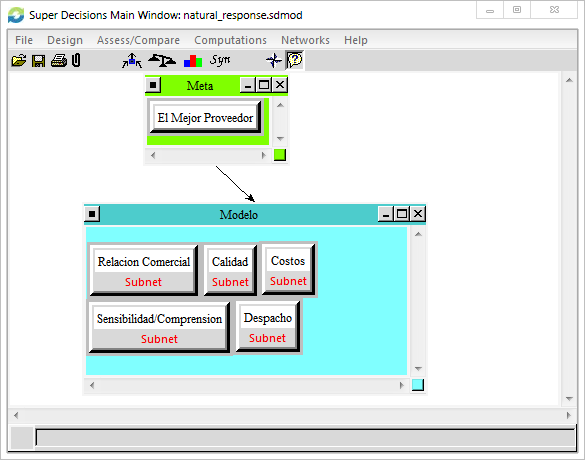
\includegraphics[width=400px]{img/1.PNG}
\end{tabular}
\caption{Modelo AHP para la primera capa de criterios}
\label{tab:modelo capa 1}
\end{table}
\newpage
\subsection{Generación de las subredes}
Luego, para cada nodo se procede a crear una subred con los subcriterios del cuadro 1, tal como se vé en la siguiente imagen:

\begin{table}[h]
\centering
\begin{tabular}{c}
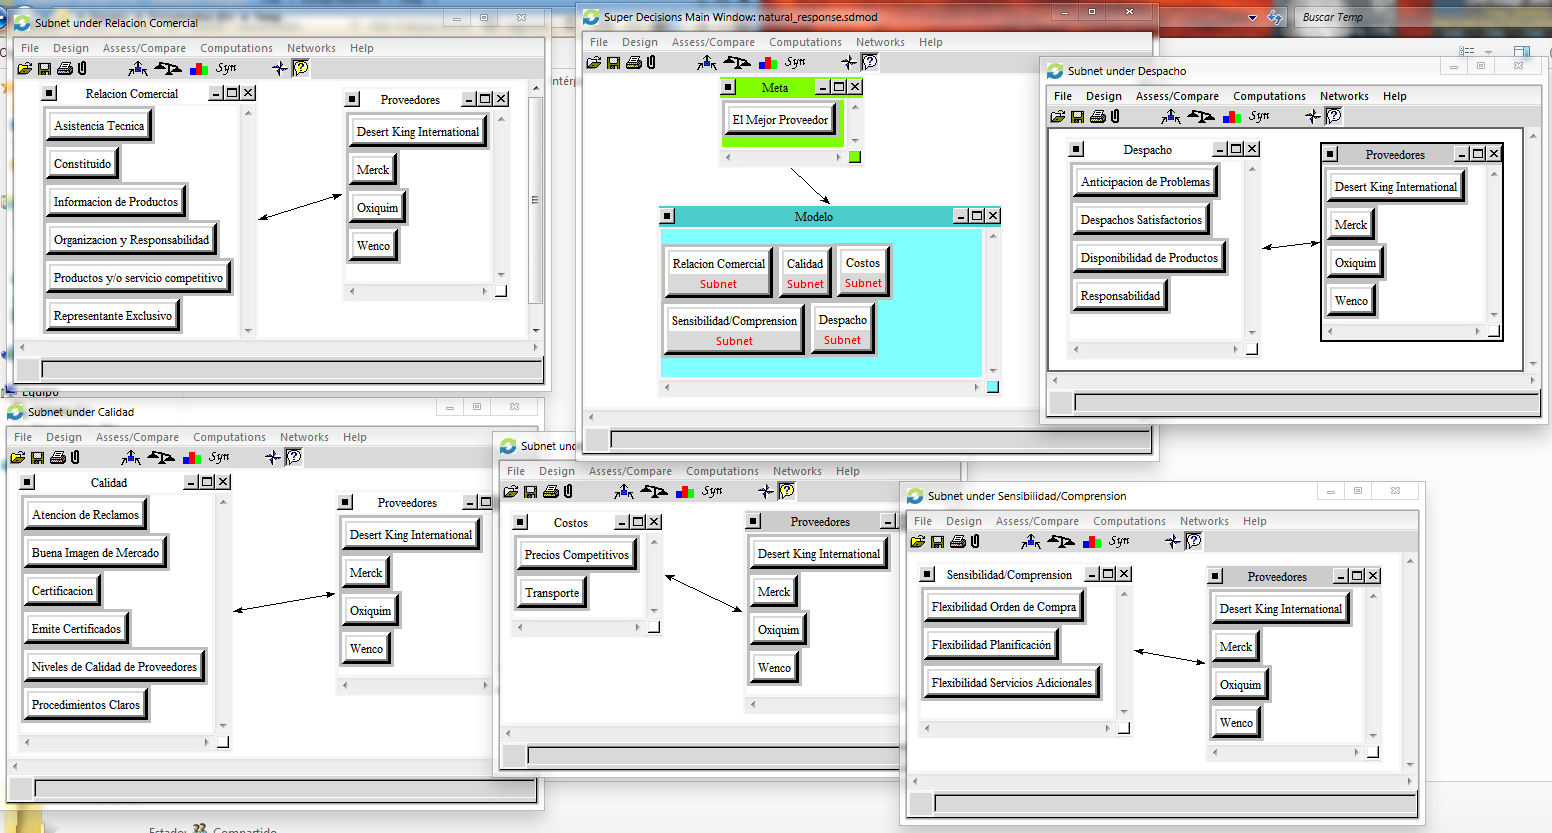
\includegraphics[width=\textwidth]{img/2.PNG}
\end{tabular}
\caption{Modelo ANP basado en BCR}
\label{tab:modelo BCR}
\end{table}

Se puede notar que en cada subred existe un nodo en común, el cual es el de los \textit{Proveedores}. Esto es escencial para el modelo, ya que es esto lo que nos permite saber cual será el mejor proveedor entre las 4 alernativas que estamos considerando.\\
Recordemos que estos proveedores actualmente se encuentra autorizados por Natural Response, pero los estudiamos para tener un punto de comparación respecto a los valores reales que estima la empresa Natural Response bajo el método AHP.
\newpage
\subsection{Comparación a pares}
Esta es básicamente la etapa más importante en el proceso del análisis bajo el método ANP, ya que necesitamos comparar cada uno de los nodos respecto a los nodos de su mismo nivel y a los nodos conectados a el. Como ya se podrá entender considerando la gran cantidad de nodos con la que cuenta nuestro modelo, estamos hablando de más de 300 combinaciones en total.\\

Podemos observar que en la siguiente imagen, las subredes han sido asignadas con los porcentajes que la empresa estima convenientes. Esto es debido a que en su modelo AHP así tienen los pesos de los árboles:

\begin{table}[h]
\centering
\begin{tabular}{c}
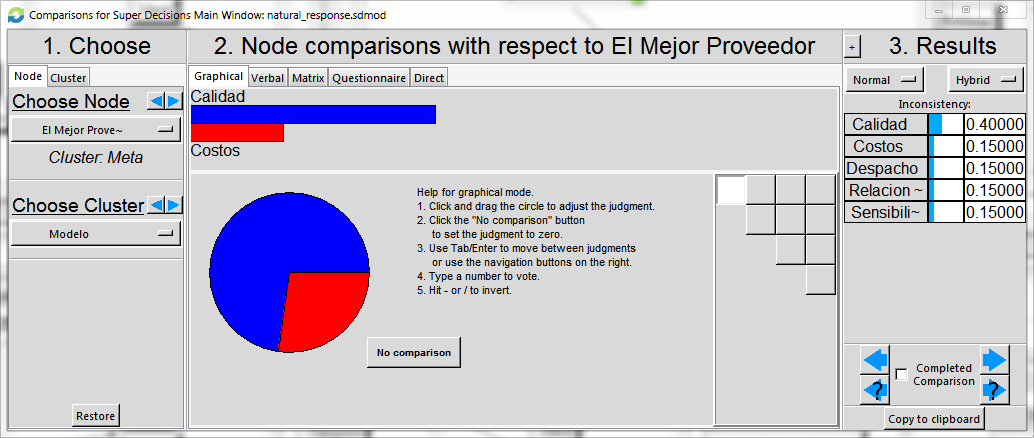
\includegraphics[width=\textwidth]{img/3.PNG}
\end{tabular}
\caption{Comparación a pares con entrada directa}
\label{tab:comparacion entrada directa}
\end{table}

Lo interesante de esto, es que el programa \textit{Super Decisions Software}, provee una completa interface para el análisis y comparación de los resultados a medida que se van llenando los datos correspondites a cada nodo. Por ejemplo, en el cuadro 4, podemos observar como el software nos muestra de manera gráfica mediante un gráfico la diferencia de la importancia entre las subredes de calidad y costos, y además entrega una guia en formato texto para entender qué es lo que significan los datos, por ejemplo: ``El nodo Calidad es considerablemente más importante que el nodo Costos".

\newpage
Para las subredes, se debe realizar la comparación a pares para cada una de las combinaciones entre las alternativas (Desert king, Merck, Oxiquim y Wenco). Para entenderlo prácticamente, verémos la comparación a pares en la subred de Costos para el nodo Transportes. Es crítico notar que el programa genera automáticamente todas las combinaciones posibles para todas las alternativas:

\begin{table}[h]
\centering
\begin{tabular}{c}
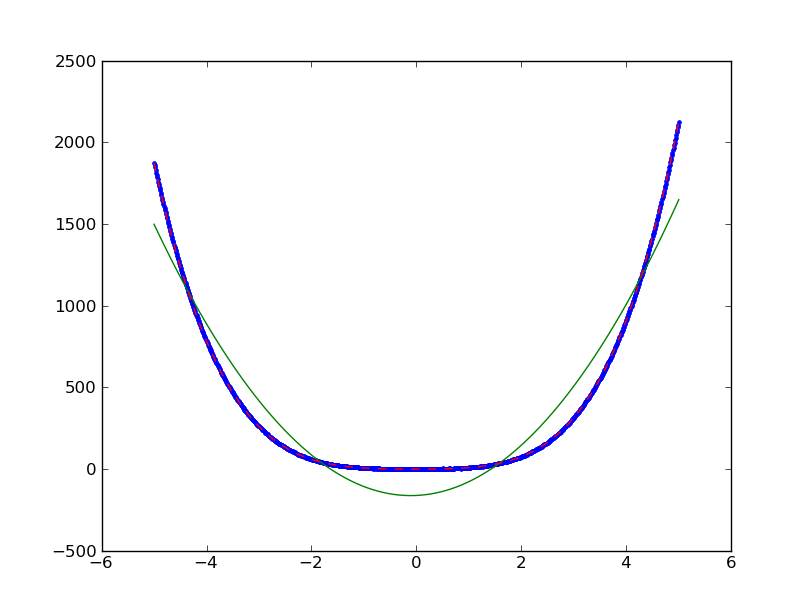
\includegraphics[width=\textwidth]{img/4.PNG}
\end{tabular}
\caption{Comparación a pares en subred}
\label{tab:comparacion a pares}
\end{table}

En este punto es válido cuestionarse \textit{¿Cómo sé que una alternativa es mejor que otra?}. La respuesta es relativa, ya que depende de la percepción de cada evaluador, y es por esto que hay que recordar que \textbf{este método solo sirve para realizar estimaciones y predicciones}.\\

Este proceso hay que repetirlo para todas los nodos existentes en todas las subredes, y rellenar con cada una de las preferencias para cada una de las alternativas y relaciones que pudiesen existir. Una vez culminado ese proceso, el software automáticamente ya ha hecho los cálculos de la mejor opción, solo nos queda revisar los resultados.\\

\textit{Tip: los nodos de alternativas en cada una de las subredes debe llamarse ``Alternatives", de este modo el programa entiende automáticamente que estamos utilizando una red de tipo BO/CR.}

\newpage
\section{Validación de Los Resultados vs. La Realidad}
A continuación comprobaremos la efectividad del método Analytic Network Process en su capacidad predictiva y de análisis. Recordemos que estamos simulando que 5 de los mejores proveedores que posee actualmente Natural Response, están intentando ingresar a ser uno de los proveedores autorizados, pero Natural Response quiere saber entre las 4 alternativas cual sería la mejor opción a incorporar.

\subsection{Resultados del método}
El programa \textit{Super Decisions Software}, tiene la capacidad de sintetizar los pesos totales entre los nodos \textit{Alternative} de cada subred, y luego los une para entregar la mejor opción. Es por esto que es de suma importancia entender a priori, que tipo de red ANP estamos modelando, ya que el software entiende automáticamente que estamos desarrollando a partir de la estructura del modelo.\\
A continuación observamos los resultados no normalizados de la red:

\begin{table}[h]
\centering
\begin{tabular}{c}
\includegraphics[width=\textwidth]{img/5.PNG}
\end{tabular}
\caption{Resultados ANP no normalizados}
\label{tab:ANP no normalizado}
\end{table}

\newpage
\subsection{Resultados de evaluaciones internas de la empresa}

\newpage
\section{Conclusión}
El Analytic Network Process es una herramienta que permite entender de mejor manera el problema que estamos enfrentando, y usado de manera correcta, puede ayudar además a resolver problemas tan complejos y delicados como la decisión de aliarse a un determinado proveedor en un gran grupo de alternativas.\\
Esto ha ayudado a mejorar el modelo que utilizaba Natural Response, y la empresa ya se encuentra interesada en desarrollar un software que permita de manera sencilla ir realizando evaluaciones periódicas de los proveedores y de proveedores que esperan a ser insertados como proveedores autorizados, ya que la empresa ha logrado entender el potencial que representa utilizar un modelo de análisis basado en redes, y que ha probado ser efectivo a la hora de mejorar el modelo existente.
\newpage
\section{Bibliografía}
\itemize
\item Saaty, Thomas L. (1996). Decision Making with Dependence and Feedback: The Analytic Network Process. Pittsburgh, Pennsylvania: RWS Publications. ISBN 0-9620317-9-8.
\item Saaty, Thomas L. (2005). \href{http://www.amazon.com/dp/1888603062}{Theory and Applications of the Analytic Network Process: Decision Making with Benefits, Opportunities, Costs and Risks. Pittsburgh, Pennsylvania: RWS Publications. ISBN 1-888603-06-2.}
\item Saaty, Thomas L.; Luis G. Vargas (2006). \href{http://www.amazon.com/dp/0387338594}{Decision Making with the Analytic Network Process: Economic, Political, Social and Technological Applications with Benefits, Opportunities, Costs and Risks. New York: Springer. ISBN 0-387-33859-4.}
\item Saaty, Thomas L.; Brady Cillo (2009). \href{http://rwspublications.com/}{The Encyclicon, Volume 2: A Dictionary of Complex Decisions using the Analytic Network Process. Pittsburgh, Pennsylvania: RWS Publications. ISBN 1-888603-09-7.}
\item Saaty, Thomas L.; Müjgan S. Özermir (2005). \href{http://www.amazon.com/dp/1888603054}{The Encyclicon: A Dictionary of Decisions with Dependence and Feedback Based on the Analytic Network Process. Pittsburgh, Pennsylvania: RWS Publications. ISBN 1-888603-05-4.}

\end{document} 